\documentclass{standalone}
\usepackage{tikz}
\usetikzlibrary{patterns, positioning}


\begin{document}
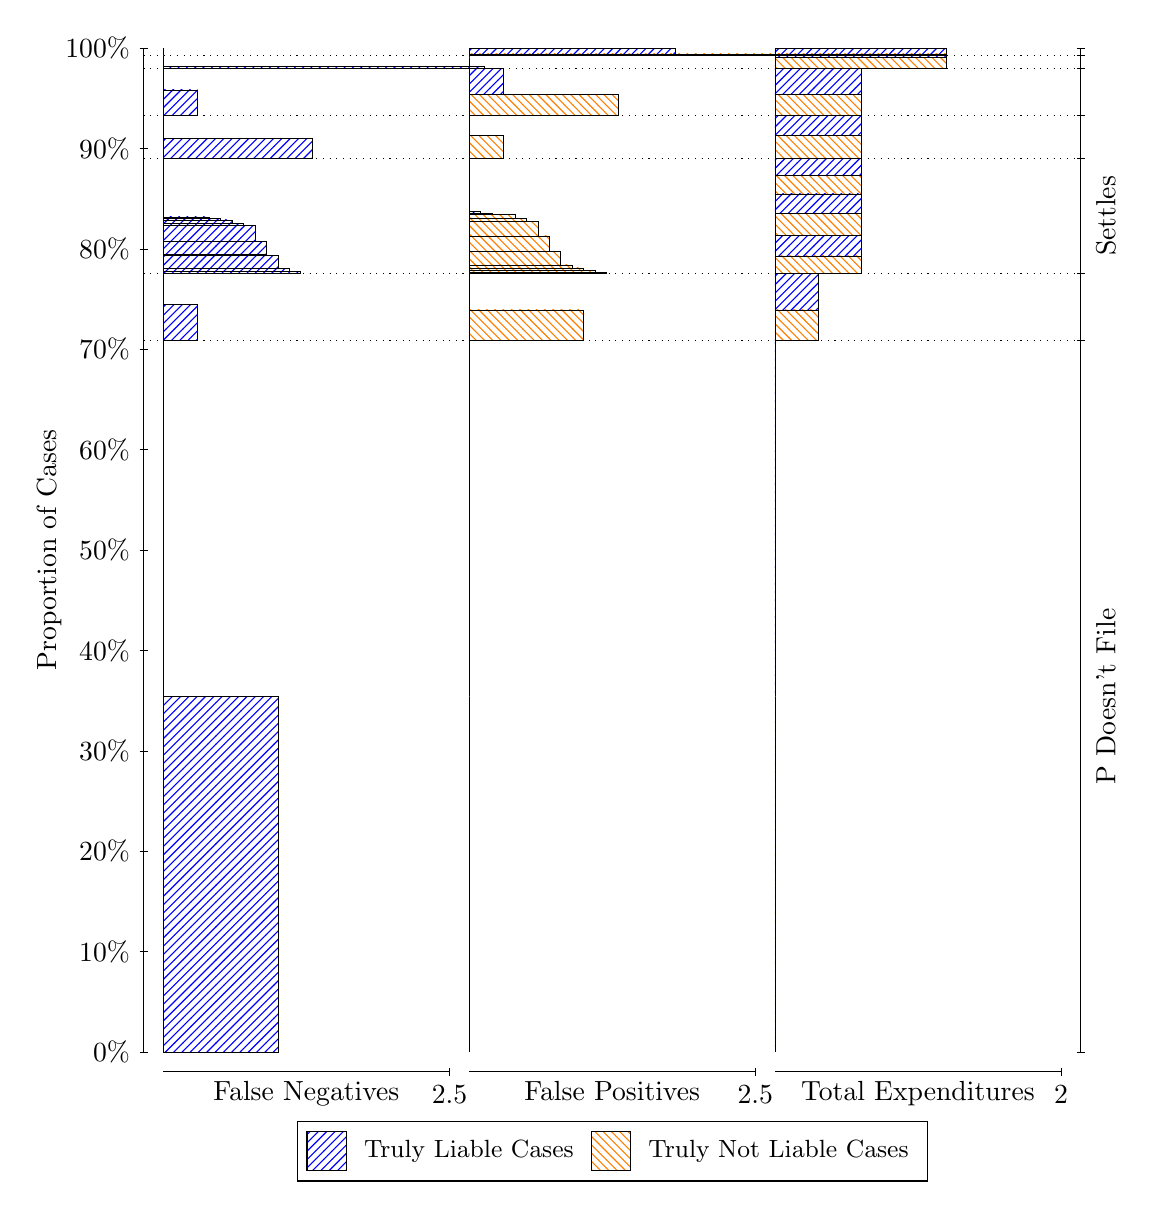
\begin{tikzpicture}
\draw[black, very thin] (1.5,1.75) -- (1.5,14.5);
\node[rotate=90, text=black, anchor=center] at (0.3, 8.125) {Proportion of Cases};
\draw[black, very thin] (1.45,1.75) -- (1.55,1.75);
\node[text=black, anchor=east] at (1.45, 1.75) {0\%};
\draw[black, very thin] (1.45,3.025) -- (1.55,3.025);
\node[text=black, anchor=east] at (1.45, 3.025) {10\%};
\draw[black, very thin] (1.45,4.3) -- (1.55,4.3);
\node[text=black, anchor=east] at (1.45, 4.3) {20\%};
\draw[black, very thin] (1.45,5.575) -- (1.55,5.575);
\node[text=black, anchor=east] at (1.45, 5.575) {30\%};
\draw[black, very thin] (1.45,6.85) -- (1.55,6.85);
\node[text=black, anchor=east] at (1.45, 6.85) {40\%};
\draw[black, very thin] (1.45,8.125) -- (1.55,8.125);
\node[text=black, anchor=east] at (1.45, 8.125) {50\%};
\draw[black, very thin] (1.45,9.4) -- (1.55,9.4);
\node[text=black, anchor=east] at (1.45, 9.4) {60\%};
\draw[black, very thin] (1.45,10.675) -- (1.55,10.675);
\node[text=black, anchor=east] at (1.45, 10.675) {70\%};
\draw[black, very thin] (1.45,11.95) -- (1.55,11.95);
\node[text=black, anchor=east] at (1.45, 11.95) {80\%};
\draw[black, very thin] (1.45,13.225) -- (1.55,13.225);
\node[text=black, anchor=east] at (1.45, 13.225) {90\%};
\draw[black, very thin] (1.45,14.5) -- (1.55,14.5);
\node[text=black, anchor=east] at (1.45, 14.5) {100\%};

\draw[black, very thin] (13.4,1.75) -- (13.4,14.5);
\draw[black, very thin] (13.35,1.75) -- (13.45,1.75);
\node[anchor=west] at (13.35, 1.75) {};
\draw[black, very thin] (13.35,10.783) -- (13.45,10.783);
\node[anchor=west] at (13.35, 10.783) {};
\draw[black, very thin] (13.35,11.636) -- (13.45,11.636);
\node[anchor=west] at (13.35, 11.636) {};
\draw[black, very thin] (13.35,13.101) -- (13.45,13.101);
\node[anchor=west] at (13.35, 13.101) {};
\draw[black, very thin] (13.35,13.64) -- (13.45,13.64);
\node[anchor=west] at (13.35, 13.64) {};
\draw[black, very thin] (13.35,14.241) -- (13.45,14.241);
\node[anchor=west] at (13.35, 14.241) {};
\draw[black, very thin] (13.35,14.403) -- (13.45,14.403);
\node[anchor=west] at (13.35, 14.403) {};
\draw[black, very thin] (13.35,14.5) -- (13.45,14.5);
\node[anchor=west] at (13.35, 14.5) {};

\draw[black, very thin, pattern color=blue, pattern=north east lines] (1.75,1.75) rectangle (3.2033,6.2665);
\draw[black, very thin, pattern color=orange, pattern=north west lines] (1.75,6.2665) rectangle (1.75,10.783);
\draw[black, very thin, pattern color=blue, pattern=north east lines] (1.75,10.783) rectangle (2.186,11.246);
\draw[black, very thin, pattern color=orange, pattern=north west lines] (1.75,11.246) rectangle (1.75,11.636);
\draw[black, very thin, pattern color=blue, pattern=north east lines] (1.75,11.636) rectangle (3.494,11.668);
\draw[black, very thin, pattern color=blue, pattern=north east lines] (1.75,11.668) rectangle (3.3487,11.697);
\draw[black, very thin, pattern color=blue, pattern=north east lines] (1.75,11.697) rectangle (3.2033,11.868);
\draw[black, very thin, pattern color=blue, pattern=north east lines] (1.75,11.868) rectangle (3.058,11.882);
\draw[black, very thin, pattern color=blue, pattern=north east lines] (1.75,11.882) rectangle (3.058,12.048);
\draw[black, very thin, pattern color=blue, pattern=north east lines] (1.75,12.048) rectangle (2.9127,12.244);
\draw[black, very thin, pattern color=blue, pattern=north east lines] (1.75,12.244) rectangle (2.7673,12.277);
\draw[black, very thin, pattern color=blue, pattern=north east lines] (1.75,12.277) rectangle (2.622,12.316);
\draw[black, very thin, pattern color=blue, pattern=north east lines] (1.75,12.316) rectangle (2.4767,12.338);
\draw[black, very thin, pattern color=blue, pattern=north east lines] (1.75,12.338) rectangle (2.3313,12.355);
\draw[black, very thin, pattern color=orange, pattern=north west lines] (1.75,12.355) rectangle (1.75,13.101);
\draw[black, very thin, pattern color=blue, pattern=north east lines] (1.75,13.101) rectangle (3.6393,13.354);
\draw[black, very thin, pattern color=orange, pattern=north west lines] (1.75,13.354) rectangle (1.75,13.64);
\draw[black, very thin, pattern color=blue, pattern=north east lines] (1.75,13.64) rectangle (2.186,13.967);
\draw[black, very thin, pattern color=orange, pattern=north west lines] (1.75,13.967) rectangle (1.75,14.241);
\draw[black, very thin, pattern color=blue, pattern=north east lines] (1.75,14.241) rectangle (5.8193,14.264);
\draw[black, very thin, pattern color=orange, pattern=north west lines] (1.75,14.264) rectangle (1.75,14.403);
\draw[black, very thin, pattern color=orange, pattern=north west lines] (1.75,14.403) rectangle (1.75,14.426);
\draw[black, very thin, pattern color=blue, pattern=north east lines] (1.75,14.426) rectangle (1.75,14.5);
\draw[black, very thin, pattern color=orange, pattern=north west lines] (5.6333,1.75) rectangle (5.6333,6.2666);
\draw[black, very thin, pattern color=blue, pattern=north east lines] (5.6333,6.2666) rectangle (5.6333,10.783);
\draw[black, very thin, pattern color=orange, pattern=north west lines] (5.6333,10.783) rectangle (7.0867,11.174);
\draw[black, very thin, pattern color=blue, pattern=north east lines] (5.6333,11.174) rectangle (5.6333,11.636);
\draw[black, very thin, pattern color=orange, pattern=north west lines] (5.6333,11.636) rectangle (7.3773,11.654);
\draw[black, very thin, pattern color=orange, pattern=north west lines] (5.6333,11.654) rectangle (7.232,11.673);
\draw[black, very thin, pattern color=orange, pattern=north west lines] (5.6333,11.673) rectangle (7.0867,11.708);
\draw[black, very thin, pattern color=orange, pattern=north west lines] (5.6333,11.708) rectangle (6.9413,11.747);
\draw[black, very thin, pattern color=orange, pattern=north west lines] (5.6333,11.747) rectangle (6.796,11.919);
\draw[black, very thin, pattern color=orange, pattern=north west lines] (5.6333,11.919) rectangle (6.6507,12.113);
\draw[black, very thin, pattern color=orange, pattern=north west lines] (5.6333,12.113) rectangle (6.5053,12.296);
\draw[black, very thin, pattern color=orange, pattern=north west lines] (5.6333,12.296) rectangle (6.36,12.337);
\draw[black, very thin, pattern color=orange, pattern=north west lines] (5.6333,12.337) rectangle (6.2147,12.383);
\draw[black, very thin, pattern color=blue, pattern=north east lines] (5.6333,12.383) rectangle (5.924,12.399);
\draw[black, very thin, pattern color=blue, pattern=north east lines] (5.6333,12.399) rectangle (5.7787,12.421);
\draw[black, very thin, pattern color=blue, pattern=north east lines] (5.6333,12.421) rectangle (5.6333,13.101);
\draw[black, very thin, pattern color=orange, pattern=north west lines] (5.6333,13.101) rectangle (6.0693,13.387);
\draw[black, very thin, pattern color=blue, pattern=north east lines] (5.6333,13.387) rectangle (5.6333,13.64);
\draw[black, very thin, pattern color=orange, pattern=north west lines] (5.6333,13.64) rectangle (7.5227,13.914);
\draw[black, very thin, pattern color=blue, pattern=north east lines] (5.6333,13.914) rectangle (6.0693,14.241);
\draw[black, very thin, pattern color=orange, pattern=north west lines] (5.6333,14.241) rectangle (5.6333,14.379);
\draw[black, very thin, pattern color=blue, pattern=north east lines] (5.6333,14.379) rectangle (5.6333,14.403);
\draw[black, very thin, pattern color=orange, pattern=north west lines] (5.6333,14.403) rectangle (9.7027,14.426);
\draw[black, very thin, pattern color=blue, pattern=north east lines] (5.6333,14.426) rectangle (8.2493,14.5);
\draw[black, very thin, pattern color=orange, pattern=north west lines] (9.5167,1.75) rectangle (9.5167,6.2666);
\draw[black, very thin, pattern color=blue, pattern=north east lines] (9.5167,6.2666) rectangle (9.5167,10.783);
\draw[black, very thin, pattern color=orange, pattern=north west lines] (9.5167,10.783) rectangle (10.062,11.174);
\draw[black, very thin, pattern color=blue, pattern=north east lines] (9.5167,11.174) rectangle (10.062,11.636);
\draw[black, very thin, pattern color=orange, pattern=north west lines] (9.5167,11.636) rectangle (10.607,11.861);
\draw[black, very thin, pattern color=blue, pattern=north east lines] (9.5167,11.861) rectangle (10.607,12.118);
\draw[black, very thin, pattern color=orange, pattern=north west lines] (9.5167,12.118) rectangle (10.607,12.401);
\draw[black, very thin, pattern color=blue, pattern=north east lines] (9.5167,12.401) rectangle (10.607,12.647);
\draw[black, very thin, pattern color=orange, pattern=north west lines] (9.5167,12.647) rectangle (10.607,12.885);
\draw[black, very thin, pattern color=blue, pattern=north east lines] (9.5167,12.885) rectangle (10.607,13.101);
\draw[black, very thin, pattern color=orange, pattern=north west lines] (9.5167,13.101) rectangle (10.607,13.387);
\draw[black, very thin, pattern color=blue, pattern=north east lines] (9.5167,13.387) rectangle (10.607,13.64);
\draw[black, very thin, pattern color=orange, pattern=north west lines] (9.5167,13.64) rectangle (10.607,13.914);
\draw[black, very thin, pattern color=blue, pattern=north east lines] (9.5167,13.914) rectangle (10.607,14.241);
\draw[black, very thin, pattern color=orange, pattern=north west lines] (9.5167,14.241) rectangle (11.697,14.379);
\draw[black, very thin, pattern color=blue, pattern=north east lines] (9.5167,14.379) rectangle (11.697,14.403);
\draw[black, very thin, pattern color=orange, pattern=north west lines] (9.5167,14.403) rectangle (11.697,14.426);
\draw[black, very thin, pattern color=blue, pattern=north east lines] (9.5167,14.426) rectangle (11.697,14.5);
\draw[black, dotted] (1.5,10.783) -- (13.4,10.783);
\draw[black, dotted] (1.5,11.636) -- (13.4,11.636);
\draw[black, dotted] (1.5,13.101) -- (13.4,13.101);
\draw[black, dotted] (1.5,13.64) -- (13.4,13.64);
\draw[black, dotted] (1.5,14.241) -- (13.4,14.241);
\draw[black, dotted] (1.5,14.403) -- (13.4,14.403);
\draw[black, very thin] (1.75,1.5) -- (5.3833,1.5);
\node[text=black, anchor=north] at (3.5667, 1.5) {False Negatives};
\draw[black, very thin] (5.3833,1.45) -- (5.3833,1.55);
\node[text=black, anchor=north] at (5.3833, 1.45) {2.5};

\draw[black, very thin] (5.6333,1.5) -- (9.2667,1.5);
\node[text=black, anchor=north] at (7.45, 1.5) {False Positives};
\draw[black, very thin] (9.2667,1.45) -- (9.2667,1.55);
\node[text=black, anchor=north] at (9.2667, 1.45) {2.5};

\draw[black, very thin] (9.5167,1.5) -- (13.15,1.5);
\node[text=black, anchor=north] at (11.333, 1.5) {Total Expenditures};
\draw[black, very thin] (13.15,1.45) -- (13.15,1.55);
\node[text=black, anchor=north] at (13.15, 1.45) {2};

\node[text=black, centered, rotate=90] at (13.72, 6.2666) {P Doesn't File};

\node[text=black, centered, rotate=90] at (13.72, 12.369) {Settles};





\draw (7.449999999999999,1.5) node[draw=none] (baseCoordinate) {};
\begin{scope}[align=center]
        \matrix[scale=0.5, draw=black, below=0.5cm of baseCoordinate, nodes={draw}, column sep=0.1cm]{
            \node[rectangle, draw, minimum width=0.5cm, minimum height=0.5cm, pattern color=blue, pattern=north east lines] {}; &
            \node[draw=none, font=\small, text=black] (B) {Truly Liable Cases}; &
            \node[rectangle, draw, minimum width=0.5cm, minimum height=0.5cm, pattern color=orange, pattern=north west lines] {}; &
            \node[draw=none, font=\small, text=black] (B) {Truly Not Liable Cases}; \\
            };
\end{scope}

\end{tikzpicture}
\end{document}